\begin{pastexam}[label={px:ncku-114-prog-13}]{成大資訊聯招 114 學年度 第 13 題}
（問答）

Considering the following graph G.

\begin{center}%
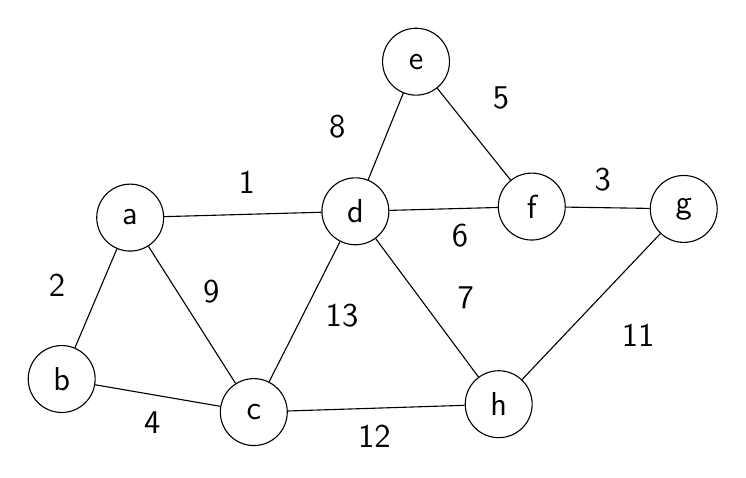
\begin{tikzpicture}[ every node/.style={font=\sffamily\large}, v/.style={circle,draw,minimum size=8.5mm,inner sep=0pt}]
\node[v] (e) at (4.50,0.00) {e};
\node[v] (a) at (0.87,-1.98) {a};
\node[v] (d) at (3.73,-1.90) {d};
\node[v] (f) at (5.97,-1.84) {f};
\node[v] (g) at (7.90,-1.87) {g};
\node[v] (b) at (0.00,-4.03) {b};
\node[v] (c) at (2.44,-4.45) {c};
\node[v] (h) at (5.55,-4.35) {h};
\draw[] (a) -- (d);
\draw[] (a) -- (b);
\draw[] (a) -- (c);
\draw[] (b) -- (c);
\draw[] (c) -- (d);
\draw[] (c) -- (h);
\draw[] (d) -- (e);
\draw[] (e) -- (f);
\draw[] (d) -- (f);
\draw[] (d) -- (h);
\draw[] (f) -- (g);
\draw[] (g) -- (h);
\node[inner sep=1pt] at (3.50,-0.82) {8};
\node[inner sep=1pt] at (5.58,-0.45) {5};
\node[inner sep=1pt] at (2.35,-1.53) {1};
\node[inner sep=1pt] at (5.06,-2.21) {6};
\node[inner sep=1pt] at (6.87,-1.50) {3};
\node[inner sep=1pt] at (-0.06,-2.84) {2};
\node[inner sep=1pt] at (1.90,-2.92) {9};
\node[inner sep=1pt] at (3.56,-3.23) {13};
\node[inner sep=1pt] at (5.13,-3.00) {7};
\node[inner sep=1pt] at (7.32,-3.48) {11};
\node[inner sep=1pt] at (1.15,-4.58) {4};
\node[inner sep=1pt] at (3.97,-4.76) {12};
\end{tikzpicture}%
\end{center}

\begin{enumerate}[label=\alph*)]
\item {[1\%]} Write out the cost of the maximum cost spanning tree for graph G.
\item {[2\%]} Write out the last edge selected into the maximum cost spanning tree for graph G when using Kruskal's method.
\item {[2\%]} Write out the 5th edge selected into the maximum cost spanning tree for graph G when using Prim's method starting with vertex a.
\end{enumerate}
\end{pastexam}

\begin{pastsoln}
答案：a) $63$。 b) 邊 $(b, c)$，權重 $4$。 c) 邊 $(d, e)$，權重 $8$。

最大成本生成樹的求法和最小生成樹一樣，只是每次挑\textbf{最重}的邊（資結書第~24.2、24.3~節；把權重取負號就是最小生成樹）。
$12$ 條邊的權重都不同，所以最大成本生成樹唯一，$8$ 個頂點要選 $7$ 條邊。

\textbf{Kruskal}：邊依權重由大到小，兩端已經連通（會成環）就跳過。
\begin{center}
\small
\begin{tabular}{rlll}
\toprule
權重 & 邊 & 結果 & 加入後的連通塊（兩個點以上的） \\
\midrule
13 & $c$--$d$ & 第 1 條 & $\{c, d\}$ \\
12 & $c$--$h$ & 第 2 條 & $\{c, d, h\}$ \\
11 & $g$--$h$ & 第 3 條 & $\{c, d, g, h\}$ \\
9 & $a$--$c$ & 第 4 條 & $\{a, c, d, g, h\}$ \\
8 & $d$--$e$ & 第 5 條 & $\{a, c, d, e, g, h\}$ \\
7 & $d$--$h$ & 跳過（$d$、$h$ 已連通） & \\
6 & $d$--$f$ & 第 6 條 & $\{a, c, d, e, f, g, h\}$ \\
5 & $e$--$f$ & 跳過 & \\
4 & $b$--$c$ & 第 7 條 & 全部 $8$ 個頂點 \\
\bottomrule
\end{tabular}
\end{center}
選滿 $7$ 條就停（$3$、$2$、$1$ 不用看，看了也都會成環）。 總成本 $13 + 12 + 11 + 9 + 8 + 6 + 4 = 63$；最後選進來的是 $(b, c)$。

\textbf{Prim，從 $a$ 開始}：每一步加入「一端在樹裡、一端不在」的邊裡最重的那一條。
\begin{center}
\small
\begin{tabular}{clll}
\toprule
第幾條 & 選的邊 & 新加入 & 當時其他的跨越邊（較重的幾條） \\
\midrule
1 & $a$--$c$（9） & $c$ & $a$--$b$ 2、$a$--$d$ 1 \\
2 & $c$--$d$（13） & $d$ & $c$--$h$ 12、$b$--$c$ 4 \\
3 & $c$--$h$（12） & $h$ & $d$--$e$ 8、$d$--$h$ 7、$d$--$f$ 6、$b$--$c$ 4 \\
4 & $g$--$h$（11） & $g$ & $d$--$e$ 8、$d$--$f$ 6、$b$--$c$ 4、$a$--$b$ 2 \\
5 & $d$--$e$（8） & $e$ & $d$--$f$ 6、$b$--$c$ 4、$f$--$g$ 3 \\
6 & $d$--$f$（6） & $f$ & $e$--$f$ 5、$b$--$c$ 4、$f$--$g$ 3 \\
7 & $b$--$c$（4） & $b$ & $a$--$b$ 2 \\
\bottomrule
\end{tabular}
\end{center}
第 $5$ 條是 $(d, e)$，權重 $8$。 Prim 得到的是同一棵樹（七條邊和 Kruskal 相同），總成本一樣是 $63$。
\end{pastsoln}
